\newpage
\section{Theorie: Kriterien zur Ideenbewertung}\label{sec:theorie}
Ideenbewertung ist in vielen Situationen wichtig. Sei es bei einer Weiterentwicklungen eines 
bereits existierenden Produkts oder aber bei innovativen Konzepten.
Durch Ideenfindungsmethoden wie zum Beispiel Brainstorming, weden sehr viele Ideen gefunden. Doch diese Ideen 
sind oft nicht alle gleich erfolgsführend. Es ist notwendig diese zu bewerten, kategoriesieren und zu durchdenken, bevor
eine Idee in die Entwicklungsphase übergeht. Dies hat besonders wirtschaftliche Gründe, denn je mehr 
Zeit vergeht, bis eine Idee als nicht umsetzbar oder nicht zielführend erkannt wird, desto mehr kostet es das Unternehmen.
Ziel der Ideenbewertung ist es, Ideen frühzeitig zu filtern um so das Risiko misslungener Investitionen zu vermeiden.
\cite{grossklaus:2008}\\
Wie \autoref{img:filterKosten} zeigt, steigen die Kosten je später eine Idee abgebrochen wird.
\begin{figure}[h]
	\centering
	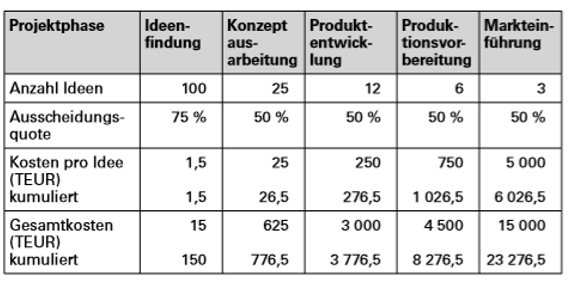
\includegraphics{ideenfilterung.png}
	\caption{Ausscheidungsquoten und Kostenentwicklung}
	\label{img:filterKosten}
\end{figure}

\subsection{Ideenbewertung}
Der Kern einer Ideenbewertung sind die Kriterien anhand derer über eine Idee geurteilt wird.
Aus diesem Grund ist wichtig, die Kriterien sorgfältig zu definieren. Werden die Kriterien falsch oder nicht sorgfältig gewält. 
Kann es zu Ablehnungsfehlern beziehungsweise Annahmefehlern kommen. 
Ablehnungsfehler bezeichnen Ideen die fälschlicherweise abgelehnt wurden, obwohl sie bei genauerer Betrachtung 
zielführend währen. Das Gegenteil sind Annahmefehler, hier wird eine Idee weiterverfolgt, obwohl diese nicht zum Ziel führt. \\
Die Kriterien lassen sich grundsätzlich in zwei Kategorien unterteilen.
\textbf{Allgemeine Kriterien} lassen sich auf verschiedene Ideen und Anwendungsfälle übertragen.
Um allgemeine Kriterien zu definieren, ist es nicht notwendig, die konkrete Aufgabe zu kennen. 
Die häufigsten allgemeinen Kriterien sind \textit{Attraktivität}, \textit{Realisierbarkeit} und 
\textit{Disruptionspotential}\\
\textbf{Aufgabenspezifische Kriterien} hingegen erfordern genaue Kenntnisse der Aufgabenstellung. Es muss klar sein, welches 
konkrete Kundenbedürfnis mit einer Idee befriedigt werden soll. Auch verschiedene Markttrends müssen hierbei beachtet werden. 
Diese haben oft entscheidenen Einfluss auf die Erfolgschancen. 

\subsection{Kriterien der Ideenbewertung nach Zephram}
Zephram teilt die Kriterien in zwei Kategorien ein. \\
\textbf{Randbedingungen} beschreiben die Eigenschaften, die eine Idee haben 
bzw. nicht haben soll. Sie sind absolut und werden oft als \textit{Muss-Kriterien}
und \textit{Darf-Nicht-Kriterien} bezeichnet.
Typische Randbedingungen sind beispielsweise die \textit{Kosten}. 
Es wird festgelegt welchen Betrag eine Ideenumsetzung maximal kosten darf. 
Weitere typische Randbedingungen sind \textit{Fit}, die Idee muss zum Unternehmen 
beziehungsweise zum Image des Unternehmens passen, oder \textit{Ressourcen}, die Ressourcen für die
Umsetzung müssen vorhanden sein. 
Randbedingungen sind entweder erfüllt oder nicht. Je nachdem wird eine Idee verworfen oder 
weiterverfolgt. \\
\textbf{Erfolgskriterien} hingegen sind nicht absolut. Sie beschreiben Eigenschaften einer Idee 
damit diese als erfolgreich gilt. Ziel ist es nicht, Ideen auszuschließen, sondern die beste bzw. 
vielversprechendste Idee heraus zu filtern. Das heißt im Umkehrschluss, alle anderen Ideen werden nicht 
verworfen, sondern zunächst nicht ausgewählt. Sie werden oft als \textit{Soll-Kriterien} bezeichnet. Um 
Erfolgskriterien einheitlich zu formulieren kann der Satz \textit{Je mehr..., desto besser"}.
Dieser Satz verdeutlicht, dass sich Erfolgskriterien nicht in erfüllt und nicht erfüllt aufteilen 
lassen. Typische Erfolgskriterien sind zum Beispiel \textit{Gewinnpotential}, \textit{Wachstumspotential} oder \textit{Kundennutzen}.\\
\textbf{Kann-Kriterien} sollten bei der Bewertung von Ideen keine Rolle spielen. Es handelt sich hierbei 
um Kriterien nicht zwingend notwendig für den Erfolg einer Idee sind. Sollte eine Idee anhand dieser Kriterien 
bewertet werden, so sind die Erfolgskriterien nicht gut gewählt und sollten demnach angepasst werden.\\
Beim \textbf{Formulieren} der Randbedingungen ist es wichtig, dass sich die Kriterien nicht
widersprechen. Sonst würden alle Ideen aussortiert werden, da niemals alle Randbedingungen erfüllt sein können.
Ein Beispiel, dass leider öfter vorkommt ist, dass eine Systemausfallsicherheit von 98\% gefordert wird, aber dass das Produkt innerhalb kurzer Zeitverfügbar ist. 
Es kommt bei den Kriterien, demnach darauf an das richtige Mittelmaß für die Aufgabe zu finden, 
deshalb sollten sollten sowohl Randbedingungen wie auch Erfolgskriterien zur Aufgabe passen. Eine weitere Schwierigkeit 
ist es eine möglichst konkrete Formulierung zu finden. \\
Beim \textbf{Anwenden} der Kriterien zur Bewertung von Ideen müssen zunächst die Randbedingungen angewandt werden. 
Dies sorgt bereits für eine starke Resuktion der Anzahl an Ideen. Um hierbei keine Fehler zu machen, wird 
ein Vier-Augen-Prinzip empfohlen. 
Schwieriger in der Anwendung sind die Erfolgskriterien, da diese graduell sind, allerdings keine klar definierte Messskala 
besitzen. Denoch gibt es einige Methoden die die Arbeit mit Erfolgskriterien vereinfachen. Einige werden 
in der folgenden Liste aufgezählt: 
\begin{itemize}
    \item Punktekleben (Siehe in Kapitel \ref{sec:retro-punkte})
    \item Nutzwertanalyse
    \item Paarvergleichsmatrix
\end{itemize}
Die Methoden die von \ac{sac} angewendet werden, werden im Praxisteil genauer beschrieben. \cite{zephram:2018}

\subsection{Vorgehensweise nach Schawel-Billing}
Vorschlag von Schawel und Billing ist die Ideenbewertung in zwei Phasen zu unterteilen. Allerdings nicht, 
wie zuvor von Zephram beschrieben in Randbedingungen und Erfolgskriterien. Zunächst muss die gesamte Anzahl 
der Ideen verringert werden. Dies geschiet in der \textbf{Ideenkategorisierung}. Hierbei geht es darum, Ideen unter 
Oberbegriffen zusammenzufassen. Dies hilft vorallem dabei, ähnliche Ideen oder Überlappungen frühzeitig zu erkennen.
Zusätzlich hat diese Vorgehensweise den Vorteil, dass die gefundenen Kategorien später in Arbeitspakete überführt werden 
könnten. Anschließend können die Kategorien in der \textbf{Ideenbewertung} genauer Bewertet werden. 
Dies erfolgt anhand formulierter Kriterien. Für eine erste Einschätzung kann außerdem eine \ac{2d}-Matrix verwendet werden. 
Diese sollte die beiden Achsen \textit{Wirkung} und \textit{Realisierbarkeit} entgegenstellen. Ideen die eine geringe Wirkung haben und/oder 
schwer zu realisieren sind können so leicht identifiziert werden. \cite{schawel:2009}